% Adapted from F05 in PR #72: same nominal geometry and colour scheme,
% but only the common initial crack is shown (no computed S1--S8 paths).
\definecolor{gTwoSoft}{rgb}{0.62,0.78,0.93}
\definecolor{gTwoStiff}{rgb}{0.93,0.68,0.60}
\definecolor{gTwoPassive}{rgb}{0.93,0.93,0.93}
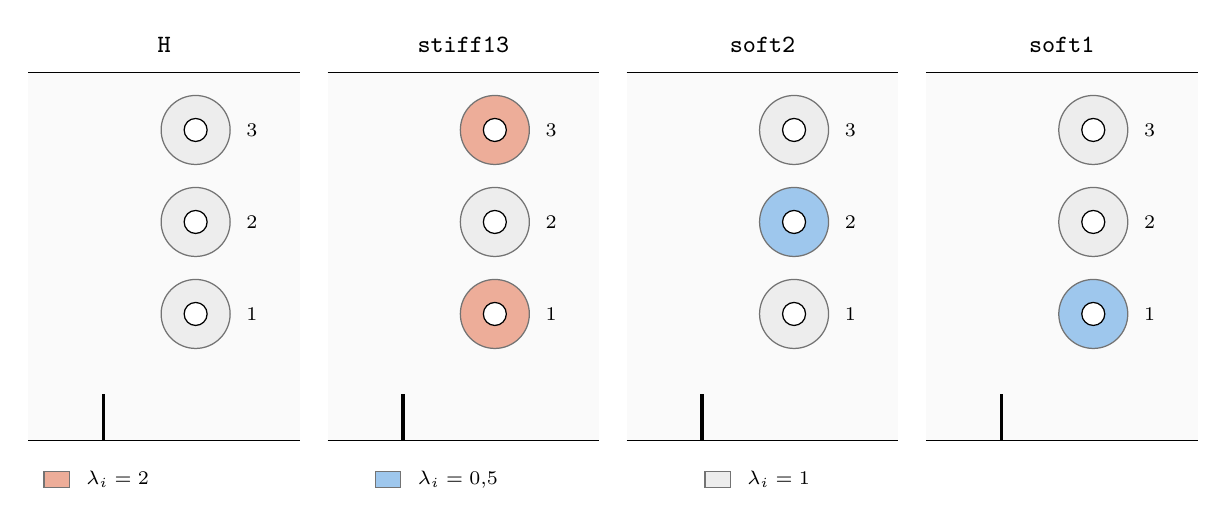
\begin{tikzpicture}[x=0.23mm,y=0.23mm,font=\small,line width=0.45pt]
  \foreach \j/\casename/\rOne/\rTwo/\rThree in {
      0/H/gTwoPassive/gTwoPassive/gTwoPassive,
      1/stiff13/gTwoStiff/gTwoPassive/gTwoStiff,
      2/soft2/gTwoPassive/gTwoSoft/gTwoPassive,
      3/soft1/gTwoSoft/gTwoPassive/gTwoPassive}{
    \begin{scope}[xshift={38mm*\j}]
      \fill[black!2] (0,0) rectangle (150,203.2);
      \draw (0,0)--(150,0) (0,203.2)--(150,203.2);
      \foreach \yy/\idx/\fc in {69.85/1/\rOne,120.65/2/\rTwo,171.45/3/\rThree}{
        \filldraw[fill=\fc,draw=black!55] (92.4,\yy) circle[radius=19.05];
        \filldraw[fill=white,draw=black] (92.4,\yy) circle[radius=6.35];
        \node[anchor=west] at (115,\yy) {\scriptsize\idx};
      }
      \draw[very thick,black] (41.6,0)--(41.6,25.4);
      \node[anchor=south] at (75,209) {\texttt{\casename}};
    \end{scope}
  }
  \begin{scope}[xshift=2mm,yshift=-6mm]
    \filldraw[fill=gTwoStiff,draw=black!55] (0,0) rectangle (14,9);
    \node[anchor=west] at (18,4.5) {\scriptsize $\lambda_i=2$};
    \filldraw[fill=gTwoSoft,draw=black!55] (183,0) rectangle (197,9);
    \node[anchor=west] at (201,4.5) {\scriptsize $\lambda_i=0{,}5$};
    \filldraw[fill=gTwoPassive,draw=black!55] (365,0) rectangle (379,9);
    \node[anchor=west] at (383,4.5) {\scriptsize $\lambda_i=1$};
  \end{scope}
\end{tikzpicture}
